
% https://www.cnblogs.com/fjlxqggc/p/15582446.html

\chapter{Variational Inference}	% 变分推断

\section{Probabilistic latent variable models} % 概率隐变量模型

\subsection{什么是隐变量模型}

概率模型的含义便是输入一组数据之后,计算这组数据的概率分布,而条件变量也类似。
而这些数据的分布可能十分复杂,并且数据内部之间存在某些关系。那么我们可以找到另一个分布
$P(z)$来表示这些数据内部的分布情况,而在这个新的分布$P(z)$的条件下,
原数据的分布就可以得到了一定的简化。

以下图中右图为例:% probabilistic_1.png

\begin{figure}[h]
\centering
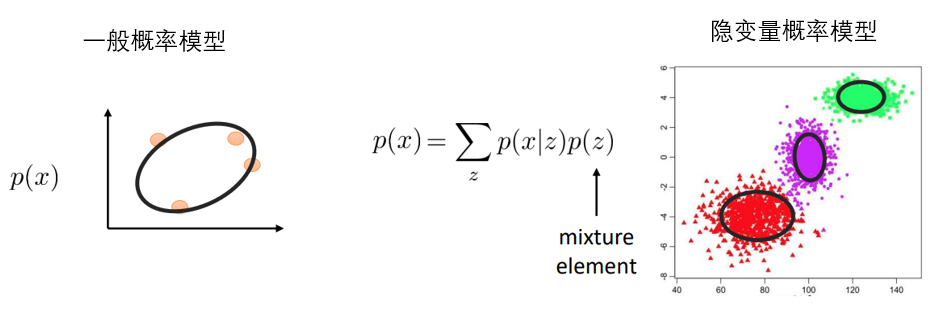
\includegraphics[scale=0.6]{pix/probabilistic_1.png}
\caption{Probabilistic Latent Variable Models}
%\label{fig:label}
\end{figure}

原数据分布$P(x)$比较复杂,但是可以看到数据内部大致形成了三类。因此可以找到一个隐变量
$z$,$Z=z_1,z_2,z_3$,在给定$z_i$的情况下,原始数据的分布为 $P(x|z_i)$,
这个分布会较为简单。而整体的数据分布可以写为:
$$
P(x)=\sum\limits_1^3P(x|z_i)P(z_i)=P(x|z_1)P(z_1)+P(x|z_2)P(z_2)+P(x|z_3)P(z_3)
$$

对于连续情况,可以将隐变量写为:$p(x)=\int p(x|z)dz$

在下图中,$p(x|z)$是多元高斯分布,均值和方差通过神经网络的输出得到,而$p(z)$
是一个简单的一维高斯分布。

\begin{figure}[h]
\centering
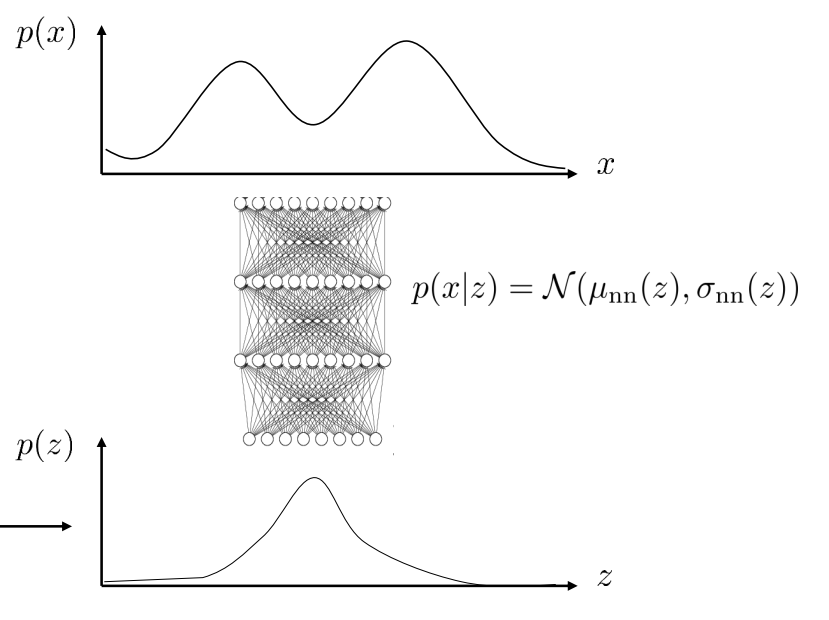
\includegraphics[scale=0.6]{pix/latent_variable.png}
\caption{Latent Variable}
%\label{fig:label}
\end{figure}


\subsection{如何训练隐变量模型}

一般的机器学习算法训练生成模型的过程中使用的是最大似然函数作为损失函数,在隐变量模型中,
将上文中重新定义的目标带入模型中可以得到新的损失函数,但此时这个损失函数是很难求解的。

\begin{figure}[h]
\centering
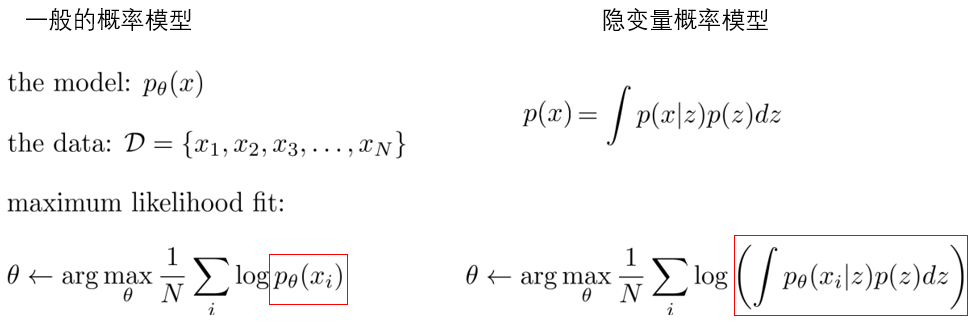
\includegraphics[scale=0.6]{pix/latent_variable_models.png}
\caption{Latent Variable Models}
%\label{fig:label}
\end{figure}

那么此时我们的问题便是如何让新的目标函数变得可以求解。可以看到此时目标函数中$z$由于是隐变量,
因此它是未知的,需要进行一些数学上的代数变形,先得到于$z$相关的一些分布之后,
才能得到整体$x$的分布。

与$z$相关的分布无非就是先验概率$p(z)$和后验概率$p(z|x_i)$,
可以将后验概率解释为给定数据$x_i$之后,这些数据的所属类别是什么。

\begin{emp_box}
{\bf\noindent
为什么会想到使用后验概率$p(z|x_i)$?}
\\
我们可以从实际的角度出发。在实际操作中,我们是先采样得到$x$,
在得到$x$后再计算$x$所属的类别$z$,即$p(z|x)$,接着基于得到的$z$通过神经网络得到$p(x|z)$,
最后计算$p(x,z)$,进而得到$p(x)$
\end{emp_box}
此时上述的损失函数就变成了:
$$
\theta \leftarrow \operatorname{argmax}_{\theta} \frac{1}{N} \sum_{i} E_{z \sim p\left(z \mid x_{i}\right)}\left[\log p_{\theta}\left(x_{i}, z\right)\right]
$$


\section{变分推断原理}

我们先推导一般概率模型中$\log\ p_\theta(x_i)$的下界:
$$
\begin{aligned}
\log p\left(x_{i}\right) &=\log \int_{z} p\left(x_{i} \mid z\right) p(z) d z \\
&=\log \int_{z} p\left(x_{i} \mid z\right) p(z) \frac{q_{i}(z)}{q_{i}(z)} d z \\
&=\log E_{z \sim q_{i}(z)}\left[\frac{p\left(x_{i} \mid z\right) p(z)}{q_{i}(z)}\right]  \\
&\geq E_{z \sim q_{i}(z)}\left[\log \frac{p\left(x_{i} \mid z\right) p(z)}{q_{i}(z)}\right] \\
&=E_{z \sim q_{i}(z)}\left[\log p\left(x_{i} \mid z\right)+\log p(z)\right]+\mathcal{H}\left(q_{i}\right)
\end{aligned}
$$

上式中倒数第二行使用了一个不等式:$\log E[\cdot]\geq E[\log(\cdot)]$,这是由于Jenson不等式。
因此原概率模型中最大似然求解就变成了最大化目前推导出来的下界,将这个下界集为$\mathcal{L}_i(p,q_i)$。
我们现在从KL散度的角度来将$q_i$和$p(z|x_i)$联系起来:
$$
\begin{aligned}
D_{\mathrm{KL}}\left(q_{i}(z) \| p\left(z \mid x_{i}\right)\right) &=E_{z \sim q_{i}(z)}\left[\log \frac{q_{i}(z)}{p\left(z \mid x_{i}\right)}\right]=E_{z \sim q_{i}(z)}\left[\log \frac{q_{i}(z) p\left(x_{i}\right)}{p\left(x_{i}, z\right)}\right] \\
&=-E_{z \sim q_{i}(z)}\left[\log p\left(x_{i} \mid z\right)+\log p(z)\right]+E_{z \sim q_{i}(z)}\left[\log q_{i}(z)\right]+E_{z \sim q_{i}(z)}\left[\log p\left(x_{i}\right)\right] \\
&=-E_{z \sim q_{i}(z)}\left[\log p\left(x_{i} \mid z\right)+\log p(z)\right]-\mathcal{H}\left(q_{i}\right)+\log p\left(x_{i}\right) \\
&=-\mathcal{L}_{i}\left(p, q_{i}\right)+\log p\left(x_{i}\right) \\
& \log p\left(x_{i}\right)=D_{\mathrm{KL}}\left(q_{i}(z) \| p\left(z \mid x_{i}\right)\right)+\mathcal{L}_{i}\left(p, q_{i}\right) \\
& \log p\left(x_{i}\right) \geq \mathcal{L}_{i}\left(p, q_{i}\right)
\end{aligned}
$$
从KL散度的角度也能看出,要最大化$\log p(x_i)$,最大化下界$\mathcal{L}_i(p,q_i)$即可。
同时我们想要下界越接近目标,就需要KL散度越接近0,因此需要$q_i(z)$接近$p(z|x_i)$。

\begin{figure}[h]
\centering
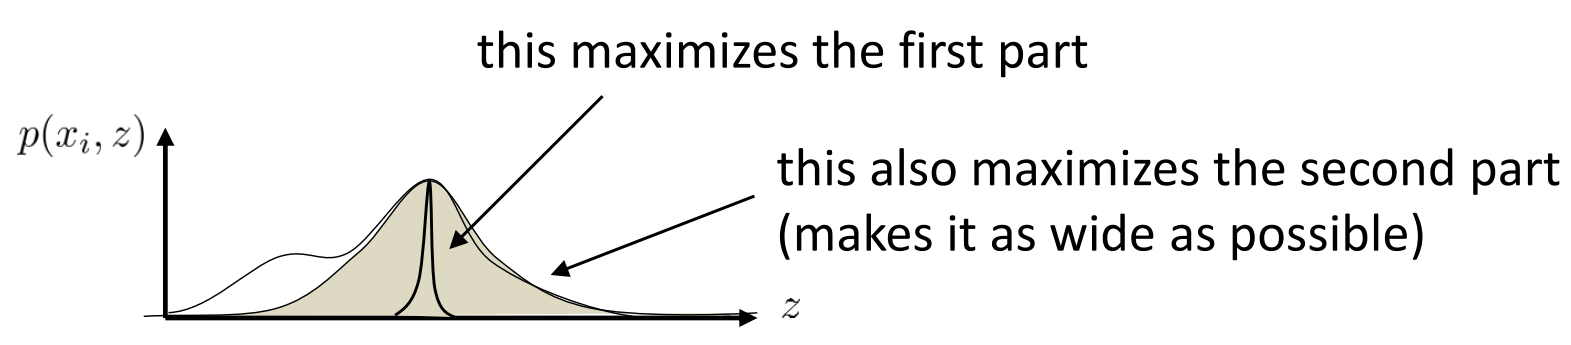
\includegraphics[scale=0.3]{pix/lost_function.png}
\caption{Lost function}
%\label{fig:label}
\end{figure}

\begin{emp_box}
现在来理解一下损失函数的两项分别是什么含义:\\
$E_{z \sim q_{i}(z)}\left[\log p\left(x_{i} \mid z\right)+\log p(z)\right]+\mathcal{H}\left(q_{i}\right)$

\noindent 其中第一项为我们的目标函数,第二项是熵(熵最大的时候为所有动作的概率都相同)。\\
\noindent 如果只考虑第一项,那我们学习到的就是窄的那个分布,这是不利于学习的。
考虑两项就能学习到中间黄色的区域。
\end{emp_box}

现在我们就可以得到一个变分推断的最基本的算法流程了:
$$
\begin{aligned}
&\text { for each }\ x_{i}\ \  (\text { or mini-batch }): \\
&\quad\quad \text { calculate } \nabla_{\theta} \mathcal{L}_{i}\left(p, q_{i}\right): \\
&\quad\quad\quad \text { sample } z \sim q_{i}(z) \\
&\quad\quad\quad \nabla_{\theta} \mathcal{L}_{i}\left(p, q_{i}\right) \approx \nabla_{\theta} \log p_{\theta}\left(x_{i} \mid z\right) \\
&\quad\theta \leftarrow \theta+\alpha \nabla_{\theta} \mathcal{L}_{i}\left(p, q_{i}\right) \\
&\quad\text { update } q_{i} \text { to maximize } \mathcal{L}_{i}\left(p, q_{i}\right)
\end{aligned}
$$
其中$q_i$的更新流程为:
$$
\begin{aligned}
&q_{i}(z)=\mathcal{N}\left(\mu_{i}, \sigma_{i}\right) \\
&\nabla_{\mu_{i}} \mathcal{L}_{i}\left(p, q_{i}\right)\ \ \text {and}\ \ \nabla_{\sigma_{i}} \mathcal{L}_{i}\left(p, q_{i}\right) \\
&\text { gradient ascent on } \mu_{i}, \sigma_{i}
\end{aligned}
$$
可以看到在上述算法中存在一个严重的问题就是需要更新的参数过多,
我们为每个样本$x_i$都拟合了一个分布$q_i$:
$$
|\theta|+(|\mu_i|+|\sigma_i|)\times N
$$
因此接下来我们就需要解决参数量过大的问题。


\section{Amortized variational inference(AVI)}

\subsection{Amortized variational inference(AVI)}

目前遇到的问题是我们为每个样本都拟合了一个分布$q_i$,
因此需要更新的参数才会随着样本的数量增大而增大。
所以我们自然而然地想到要对这个$q_i$进行修改,
这里想到的方法是使用一个单独的神经网络来输出每个样本需要的$\mu_i$,$\sigma_i$,
这也就是`amortized`所表达的意思。




